%%%%%%%%%%%%%%%%%%%%%%%%%%%%%%%%%%%%%%%%%
% Programming/Coding Assignment
% LaTeX Template
%
% This template has been downloaded from:
% http://www.latextemplates.com
%
% Original author:
% Ted Pavlic (http://www.tedpavlic.com)
%
% Note:
% The \lipsum[#] commands throughout this template generate dummy text
% to fill the template out. These commands should all be removed when 
% writing assignment content.
%
% This template uses a Perl script as an example snippet of code, most other
% languages are also usable. Configure them in the "CODE INCLUSION 
% CONFIGURATION" section.
%
%%%%%%%%%%%%%%%%%%%%%%%%%%%%%%%%%%%%%%%%%

%----------------------------------------------------------------------------------------
%	PACKAGES AND OTHER DOCUMENT CONFIGURATIONS
%----------------------------------------------------------------------------------------

\documentclass{article}

\usepackage{fancyhdr} % Required for custom headers
\usepackage{lastpage} % Required to determine the last page for the footer
\usepackage{extramarks} % Required for headers and footers
\usepackage[usenames,dvipsnames]{color} % Required for custom colors
\usepackage{graphicx} % Required to insert images
\usepackage{listings} % Required for insertion of code
\usepackage{courier} % Required for the courier font
\usepackage{lipsum} % Used for inserting dummy 'Lorem ipsum' text into the template
\usepackage{natbib}
\usepackage{hyperref}


% Margins
\topmargin=-0.45in
\evensidemargin=0in
\oddsidemargin=0in
\textwidth=6.5in
\textheight=9.0in
\headsep=0.25in

\linespread{1.1} % Line spacing

% Set up the header and footer
\pagestyle{fancy}
\lhead{\hmwkAuthorName} % Top left header
\chead{\hmwkClass\ (\hmwkClassInstructor\ \hmwkClassTime): \hmwkTitle} % Top center head
\rhead{\firstxmark} % Top right header
\lfoot{\lastxmark} % Bottom left footer
\cfoot{} % Bottom center footer
\rfoot{Page\ \thepage\ of\ \protect\pageref{LastPage}} % Bottom right footer
\renewcommand\headrulewidth{0.4pt} % Size of the header rule
\renewcommand\footrulewidth{0.4pt} % Size of the footer rule

\setlength\parindent{0pt} % Removes all indentation from paragraphs

%----------------------------------------------------------------------------------------
%	CODE INCLUSION CONFIGURATION
%----------------------------------------------------------------------------------------

\definecolor{MyDarkGreen}{rgb}{0.0,0.4,0.0} % This is the color used for comments
\lstloadlanguages{Perl} % Load Perl syntax for listings, for a list of other languages supported see: ftp://ftp.tex.ac.uk/tex-archive/macros/latex/contrib/listings/listings.pdf
\lstset{language=Perl, % Use Perl in this example
        frame=single, % Single frame around code
        basicstyle=\small\ttfamily, % Use small true type font
        keywordstyle=[1]\color{Blue}\bf, % Perl functions bold and blue
        keywordstyle=[2]\color{Purple}, % Perl function arguments purple
        keywordstyle=[3]\color{Blue}\underbar, % Custom functions underlined and blue
        identifierstyle=, % Nothing special about identifiers                                         
        commentstyle=\usefont{T1}{pcr}{m}{sl}\color{MyDarkGreen}\small, % Comments small dark green courier font
        stringstyle=\color{Purple}, % Strings are purple
        showstringspaces=false, % Don't put marks in string spaces
        tabsize=5, % 5 spaces per tab
        %
        % Put standard Perl functions not included in the default language here
        morekeywords={rand},
        %
        % Put Perl function parameters here
        morekeywords=[2]{on, off, interp},
        %
        % Put user defined functions here
        morekeywords=[3]{test},
       	%
        morecomment=[l][\color{Blue}]{...}, % Line continuation (...) like blue comment
        numbers=left, % Line numbers on left
        firstnumber=1, % Line numbers start with line 1
        numberstyle=\tiny\color{Blue}, % Line numbers are blue and small
        stepnumber=5, % Line numbers go in steps of 5
        breaklines = True
}

% Creates a new command to include a perl script, the first parameter is the filename of the script (without .pl), the second parameter is the caption
\newcommand{\pythonscript}[2]{
\begin{itemize}
\item[]\lstinputlisting[caption=#2,label=#1]{#1.py}
\end{itemize}
}

%----------------------------------------------------------------------------------------
%	DOCUMENT STRUCTURE COMMANDS
%	Skip this unless you know what you're doing
%----------------------------------------------------------------------------------------

% Header and footer for when a page split occurs within a problem environment
\newcommand{\enterProblemHeader}[1]{
\nobreak\extramarks{#1}{#1 continued on next page\ldots}\nobreak
\nobreak\extramarks{#1 (continued)}{#1 continued on next page\ldots}\nobreak
}

% Header and footer for when a page split occurs between problem environments
\newcommand{\exitProblemHeader}[1]{
\nobreak\extramarks{#1 (continued)}{#1 continued on next page\ldots}\nobreak
\nobreak\extramarks{#1}{}\nobreak
}

\setcounter{secnumdepth}{0} % Removes default section numbers
\newcounter{homeworkProblemCounter} % Creates a counter to keep track of the number of problems

\newcommand{\homeworkProblemName}{}
\newenvironment{homeworkProblem}[1][Problem \arabic{homeworkProblemCounter}]{ % Makes a new environment called homeworkProblem which takes 1 argument (custom name) but the default is "Problem #"
\stepcounter{homeworkProblemCounter} % Increase counter for number of problems
\renewcommand{\homeworkProblemName}{#1} % Assign \homeworkProblemName the name of the problem
\section{\homeworkProblemName} % Make a section in the document with the custom problem count
\enterProblemHeader{\homeworkProblemName} % Header and footer within the environment
}{
\exitProblemHeader{\homeworkProblemName} % Header and footer after the environment
}

\newcommand{\problemAnswer}[1]{ % Defines the problem answer command with the content as the only argument
\noindent\framebox[\columnwidth][c]{\begin{minipage}{0.98\columnwidth}#1\end{minipage}} % Makes the box around the problem answer and puts the content inside
}

\newcommand{\homeworkSectionName}{}
\newenvironment{homeworkSection}[1]{ % New environment for sections within homework problems, takes 1 argument - the name of the section
\renewcommand{\homeworkSectionName}{#1} % Assign \homeworkSectionName to the name of the section from the environment argument
\subsection{\homeworkSectionName} % Make a subsection with the custom name of the subsection
\enterProblemHeader{\homeworkProblemName\ [\homeworkSectionName]} % Header and footer within the environment
}{
\enterProblemHeader{\homeworkProblemName} % Header and footer after the environment
}

%----------------------------------------------------------------------------------------
%	NAME AND CLASS SECTION
%----------------------------------------------------------------------------------------

\newcommand{\hmwkTitle}{Assignment\ \#3} % Assignment title
\newcommand{\hmwkDueDate}{Thursday,\ April\ 2,\ 2015} % Due date
\newcommand{\hmwkClass}{CS\ 851} % Course/class
\newcommand{\hmwkClassTime}{4:20PM} % Class/lecture time
\newcommand{\hmwkClassInstructor}{DR NELSON} % Teacher/lecturer
\newcommand{\hmwkAuthorName}{VICTOR NWALA} % Your name

%----------------------------------------------------------------------------------------
%	TITLE PAGE
%----------------------------------------------------------------------------------------

\title{
\vspace{2in}
\textmd{\textbf{\hmwkClass:\ \hmwkTitle}}\\
\normalsize\vspace{0.1in}\small{Due\ on\ \hmwkDueDate}\\
\vspace{0.1in}\large{\textit{\hmwkClassInstructor\ \hmwkClassTime}}
\vspace{3in}
}

\author{\textbf{\hmwkAuthorName}}
\date{} % Insert date here if you want it to appear below your name

%----------------------------------------------------------------------------------------

\begin{document}

\maketitle

%----------------------------------------------------------------------------------------
%	TABLE OF CONTENTS
%----------------------------------------------------------------------------------------

%\setcounter{tocdepth}{1} % Uncomment this line if you don't want subsections listed in the ToC

\newpage
\tableofcontents
\newpage

%----------------------------------------------------------------------------------------
%	PROBLEM 1
%----------------------------------------------------------------------------------------

% To have just one problem per page, simply put a \clearpage after each problem

\begin{homeworkProblem}
For the text you saved for the 10000 URIs from A1, Q2:
\newline
Use the “boilerpipe” software to remove the HTML templates from all HTML pages (document how many pages link from the tweets were non-HTML and had to be skipped)
\newline
https://code.google.com/p/boilerpipe/ 
\newline
WSDM 2010 paper: http://www.l3s.de/~kohlschuetter/boilerplate/
\newline
For how many of the 10000 URIs was boilerpipe successful? 
\newline
Compare the total words, unique words, and byte sizes before and after use of boilerpipe
\newline
For what classes of pages was it successful? 
\newline 
For what classes of pages was it unsuccessful?
\newline
Provide examples of both successful and unsuccessful removals and discuss at length. 
\newline
To answer this question, I started with 10000 links, only 910 of them were unique links, after I used justext to extract my text files only 53 links were successful. 
\newline
I answered my question in a different way, I extracted my text files with justext, I took note of the successful links and inturn extracted the html pages from those links using wget.
\newline
The classes of pages that were succesful 200 OK pages, html pages. The classes of unsucessful pages were, 404 response pages, pages with all the different kinds of redirects i.e. 301, 302, etc. 
\newline
The text files have 4025 unique words and a total of 27870 words and a combined size of 174.8kb. The html files have a total of 22931 unique words and a total of 63253 words and a combined size of 985.5kb. Note this for html files, it includes non-english characters.



\pythonscript{pipeBoiler}{Python script to extract text files from URIs using justext}

\pythonscript{downloadPage}{Python script to extract html files from URIs using wget}

\pythonscript{remove}{Python script to eliminate duplicate URIs}

\pythonscript{combine}{Python script to combine text files into one file}




\end{homeworkProblem}

%----------------------------------------------------------------------------------------
%	PROBLEM 2
%----------------------------------------------------------------------------------------

\begin{homeworkProblem}

Collection1: Extract all the unique terms and their frequency from the 10000 files*
\newline
Collection2: Extract all the unique terms and their frequency of the 10000 files* after running boilerpipe
\newline
Construct a table with the top 50 terms from each collection. 
\newline
Find a common stop word list.  How many of the 50 terms are on that stop word list?
\newline
For both collections, construct a graph with the x-axis as word rank, and y-axis as word frequency.  
\newline
Do either follow a Zipf distribution? Support your answer.

\pythonscript{wordcount}{Python script used to extract and count unique words and their frequencies for justext text files credits to Thiago Marzagao }

\pythonscript{html2text}{Python script used to extract and count unique words and their frequencies for html text files}

\newpage

\begin {table}[H]
\caption{ Word, Rank and Frequency From HTML File}
\centering
\scalebox{0.9}{
  \begin{tabular}{ l | c || r }
    \hline
    RANK & WORD & FREQUENCY \\ \hline
1 & the & 1307 \\ \hline
2 & to & 1065 \\ \hline
3 & and & 788 \\ \hline
4 & of & 675 \\ \hline
5 & a & 638 \\ \hline
6 & in & 561 \\ \hline
7 & at  & 414 \\ \hline
8 & for &   410 \\ \hline
9 & by  & 378 \\ \hline
10 & is & 340 \\ \hline
11 & i  & 334 \\ \hline
12 & on & 328 \\ \hline
13 & with & 308 \\ \hline
14 & you    & 294 \\ \hline
15 & that   & 268 \\ \hline
16 & your   & 262 \\ \hline
17 & this   & 249 \\ \hline
18 & posted & 223 \\ \hline
19 & 2015   & 194 \\ \hline
20 & it & 191 \\ \hline
21 & o  & 189 \\ \hline
22 & 2015年02月04日  & 157 \\ \hline
23 & from   & 151 \\ \hline
24 & as & 145 \\ \hline
25 & or & 142 \\ \hline
26 & are    & 140 \\ \hline
27 & |  & 140 \\ \hline
28 & have   & 134 \\ \hline
29 &my  & 127 \\ \hline
30 &all & 124 \\ \hline
31 & be & 118 \\ \hline
32 & not    & 114 \\ \hline
33 & can    & 111 \\ \hline
34 & new    & 109 \\ \hline
35 & published  & 106 \\ \hline
36 & out    & 104 \\ \hline
37 & more   & 100 \\ \hline
38 & will   & 90 \\ \hline
39 & an & 88 \\ \hline
40 & get    & 86 \\ \hline
41 & has    & 84 \\ \hline
42 & one    & 83 \\ \hline
43 & was    & 83 \\ \hline
44 & like   & 81 \\ \hline
45 & about  & 80 \\ \hline
46 & her    & 80 \\ \hline
47 & but    & 79 \\ \hline
48 & up & 71 \\ \hline
49 & when   & 71 \\ \hline
50 & march  & 68 \\ \hline
   \hline
  \end{tabular}
  }
\end {table}


\begin {table}[H]
\caption{ Word, Rank and Frequency From Justext File}
\begin{center}
\scalebox{0.9}{
  \begin{tabular}{ l | c || r }
    \hline
    RANK & WORD & FREQUENCY \\ \hline
1 & the  &  1288 \\ \hline
2 & to & 1057 \\ \hline
3 & and & 809 \\ \hline
4 & of & 635 \\ \hline
5 & a  & 623 \\ \hline
6 & you & 468 \\ \hline
7 & in & 410 \\ \hline
8 & is & 335 \\ \hline
9 & that  & 304 \\ \hline
10 & i  & 289 \\ \hline
11 & for & 280 \\ \hline
12 & it &  253 \\ \hline
13 & with  &  249 \\ \hline
14 & or & 245 \\ \hline
15 & on & 229 \\ \hline
16 & this & 222 \\ \hline
17 & we & 221 \\ \hline
18 & s  & 218 \\ \hline
19 & your  & 201 \\ \hline
20 & as & 176 \\ \hline
21 & from &   170 \\ \hline
22 & information & 160 \\ \hline
23 & will   & 158 \\ \hline
24 & are & 156 \\ \hline
25 & not & 151 \\ \hline
26 & by & 141 \\ \hline
27 & be & 140 \\ \hline
28 & at & 135 \\ \hline
29 & have &  133 \\ \hline
30 & plndr  & 120 \\ \hline
31 & can & 116 \\ \hline
32 & my & 107 \\ \hline
33 & t &  102 \\ \hline
34 & an & 97 \\ \hline
35 & if & 95 \\ \hline
36 & when &  93 \\ \hline
37 & our & 92 \\ \hline
38 & use & 91 \\ \hline
39 & so & 90 \\ \hline
40 & more & 83 \\ \hline
41 & but & 81\\ \hline
42 & do & 78 \\ \hline
43 & any & 77 \\ \hline
44 & about & 77 \\ \hline
45 & her & 74 \\ \hline
46 & new & 71 \\ \hline
47 & us & 69 \\ \hline
48 & may & 69 \\ \hline
49 & time & 68 \\ \hline
50 & their &  68 \\
    \hline
  \end{tabular}
  }
\end{center}
\end {table}





\begin{center}
{Figure 1: GRAPH OF WORDRANK VS FREQUENCY FOR TEXT}
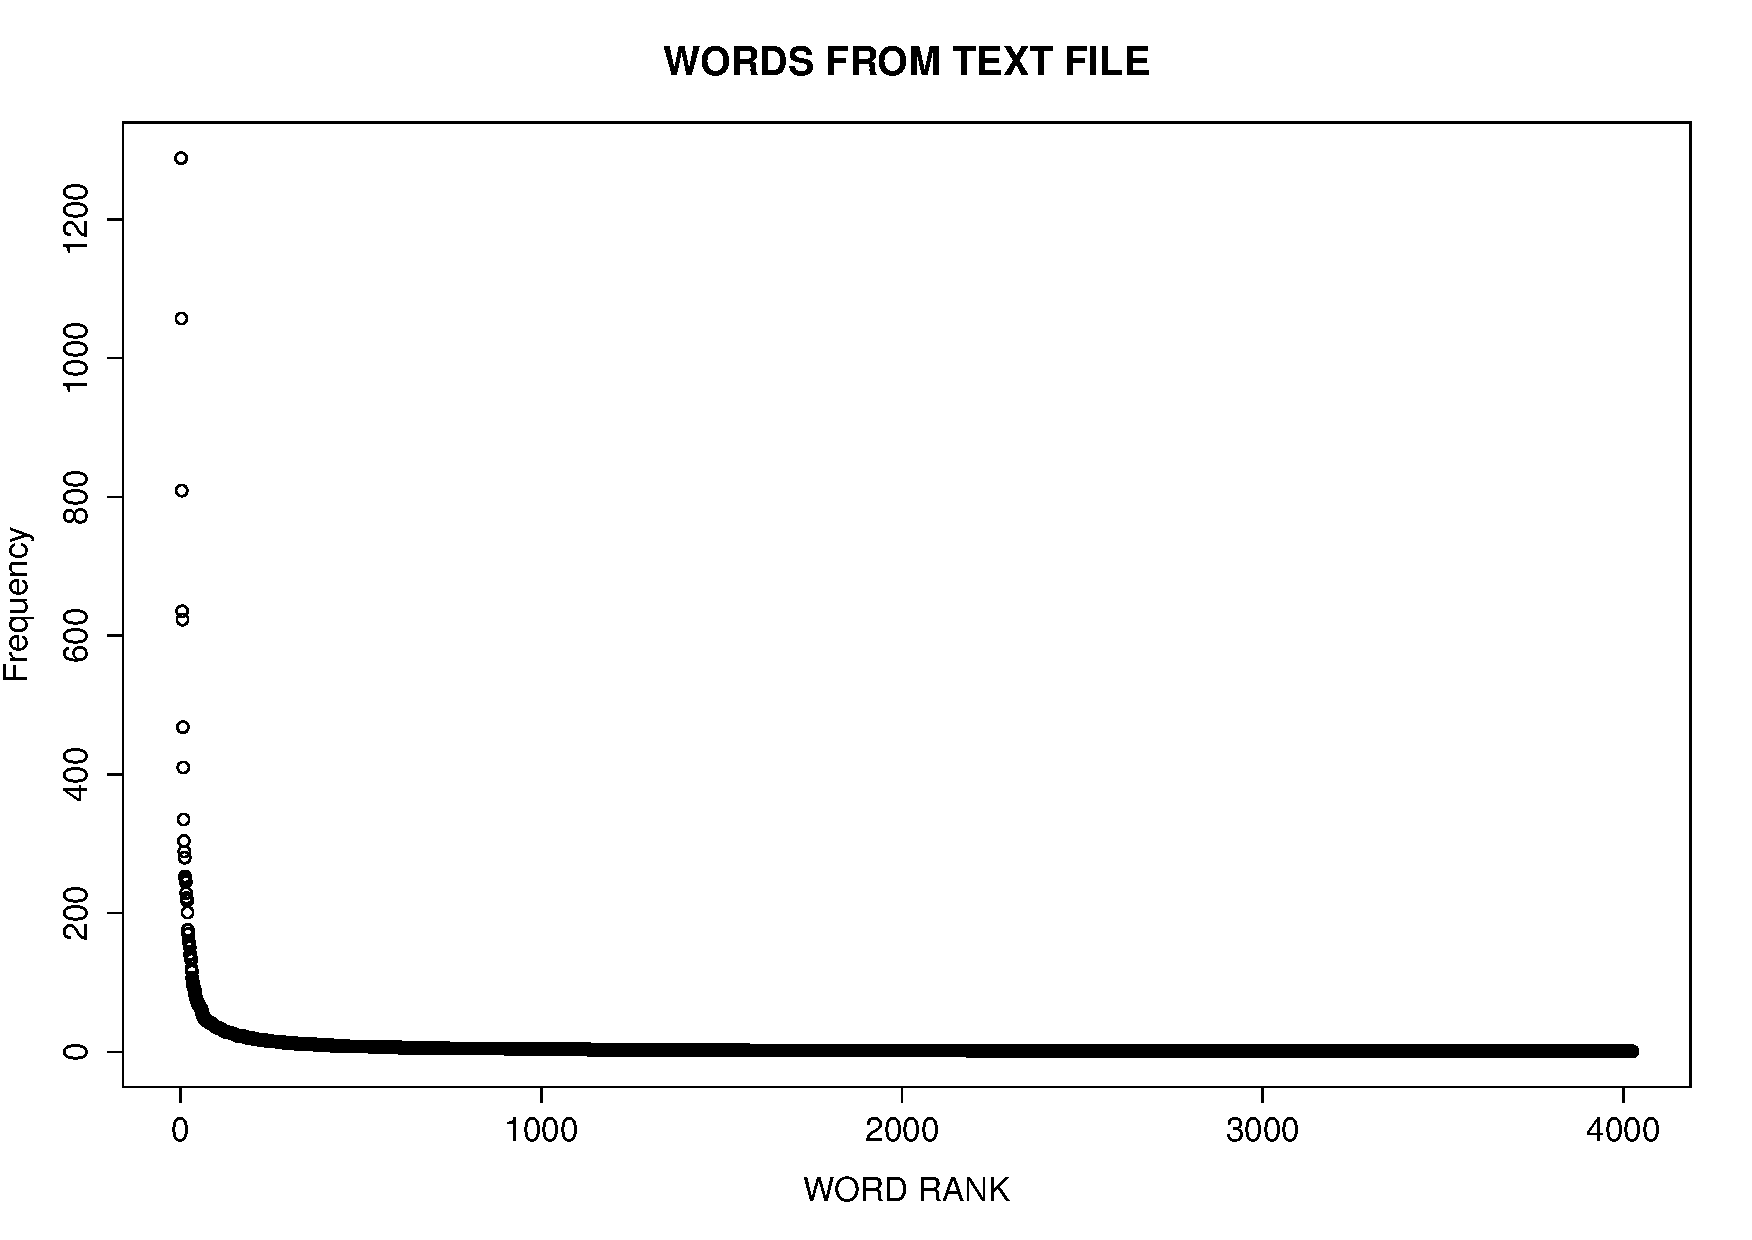
\includegraphics[width=0.8\columnwidth]{RplotText} % Example image
\end{center}



\begin{center}
{Figure 2: GRAPH OF WORDRANK VS FREQUENCY FOR HTML-TEXT}
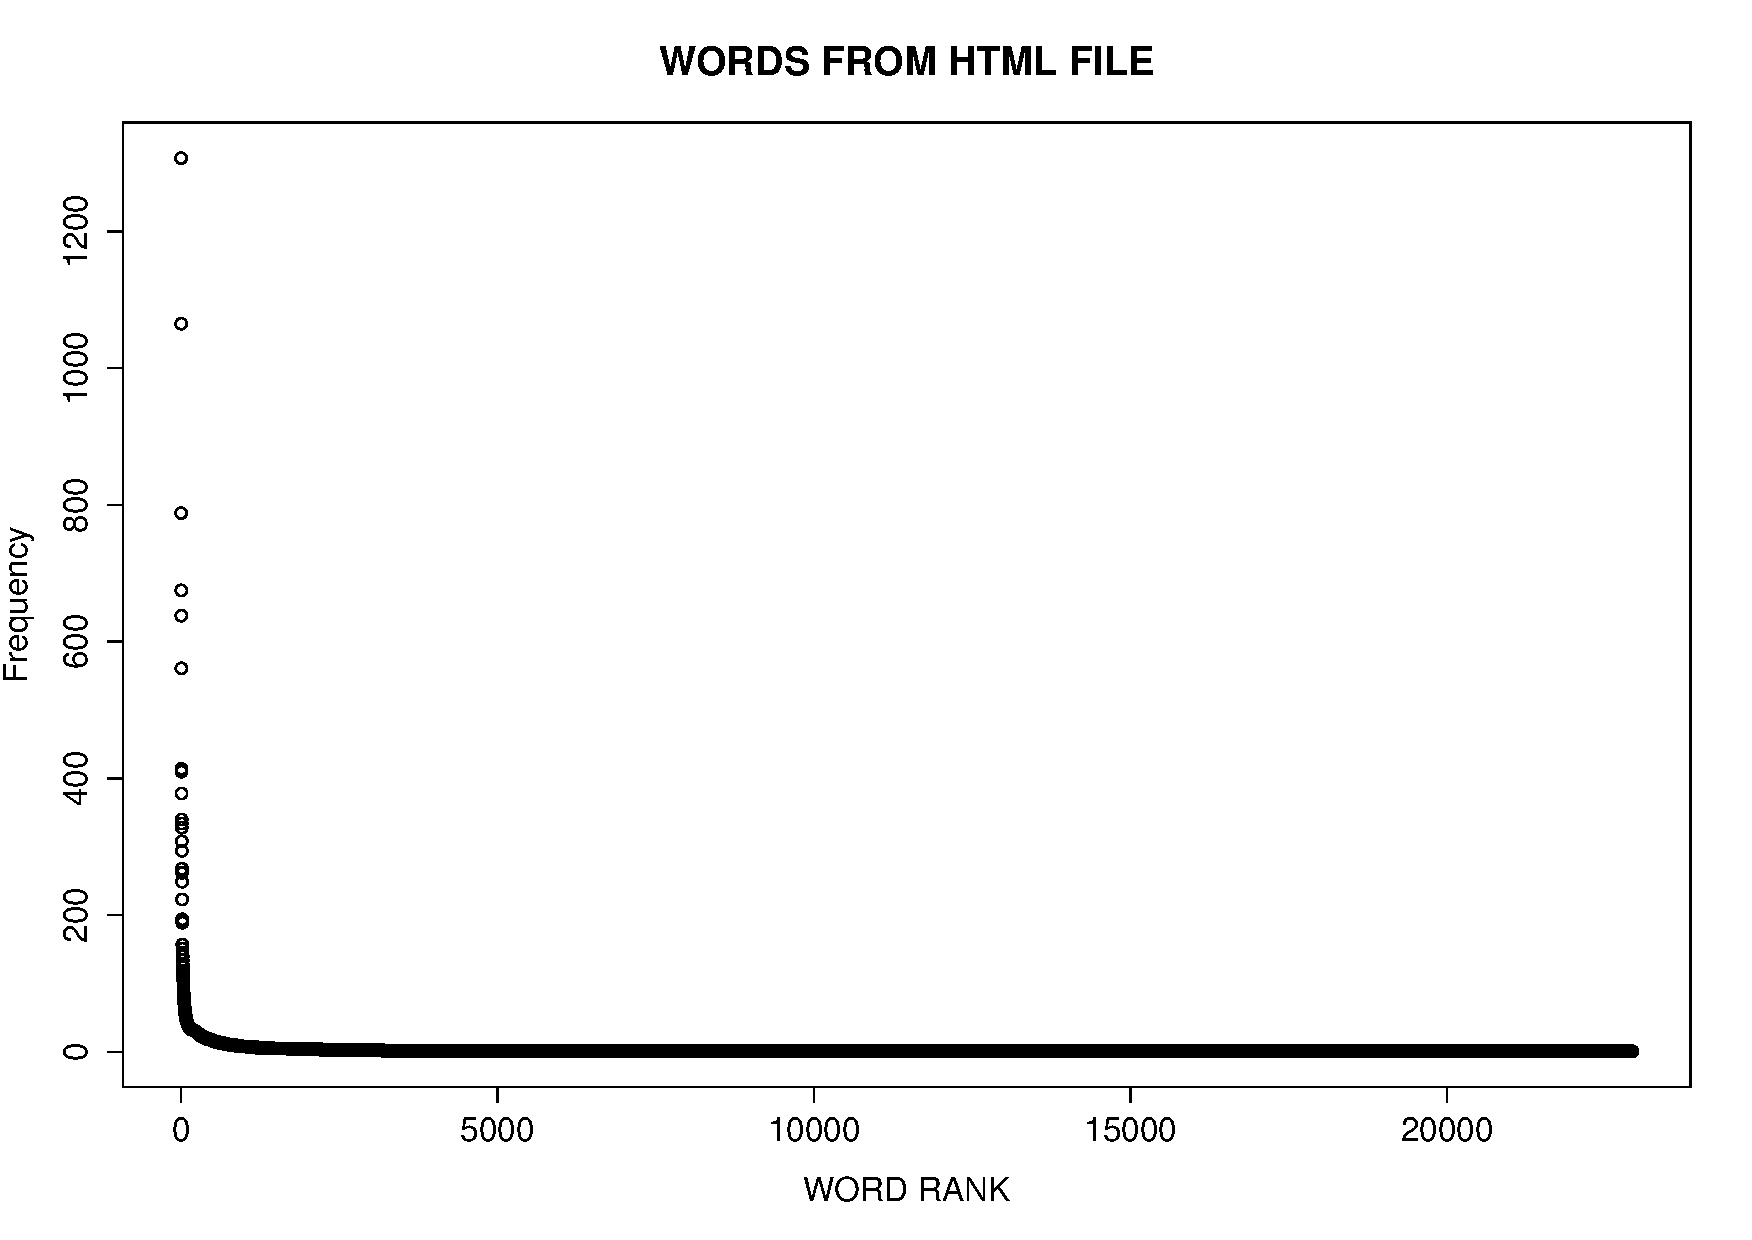
\includegraphics[width=0.8\columnwidth]{RplotHtml} % Example image
\end{center}


\begin{center}
{Figure 3: GRAPH TO PROVE Zipf’s LAW}
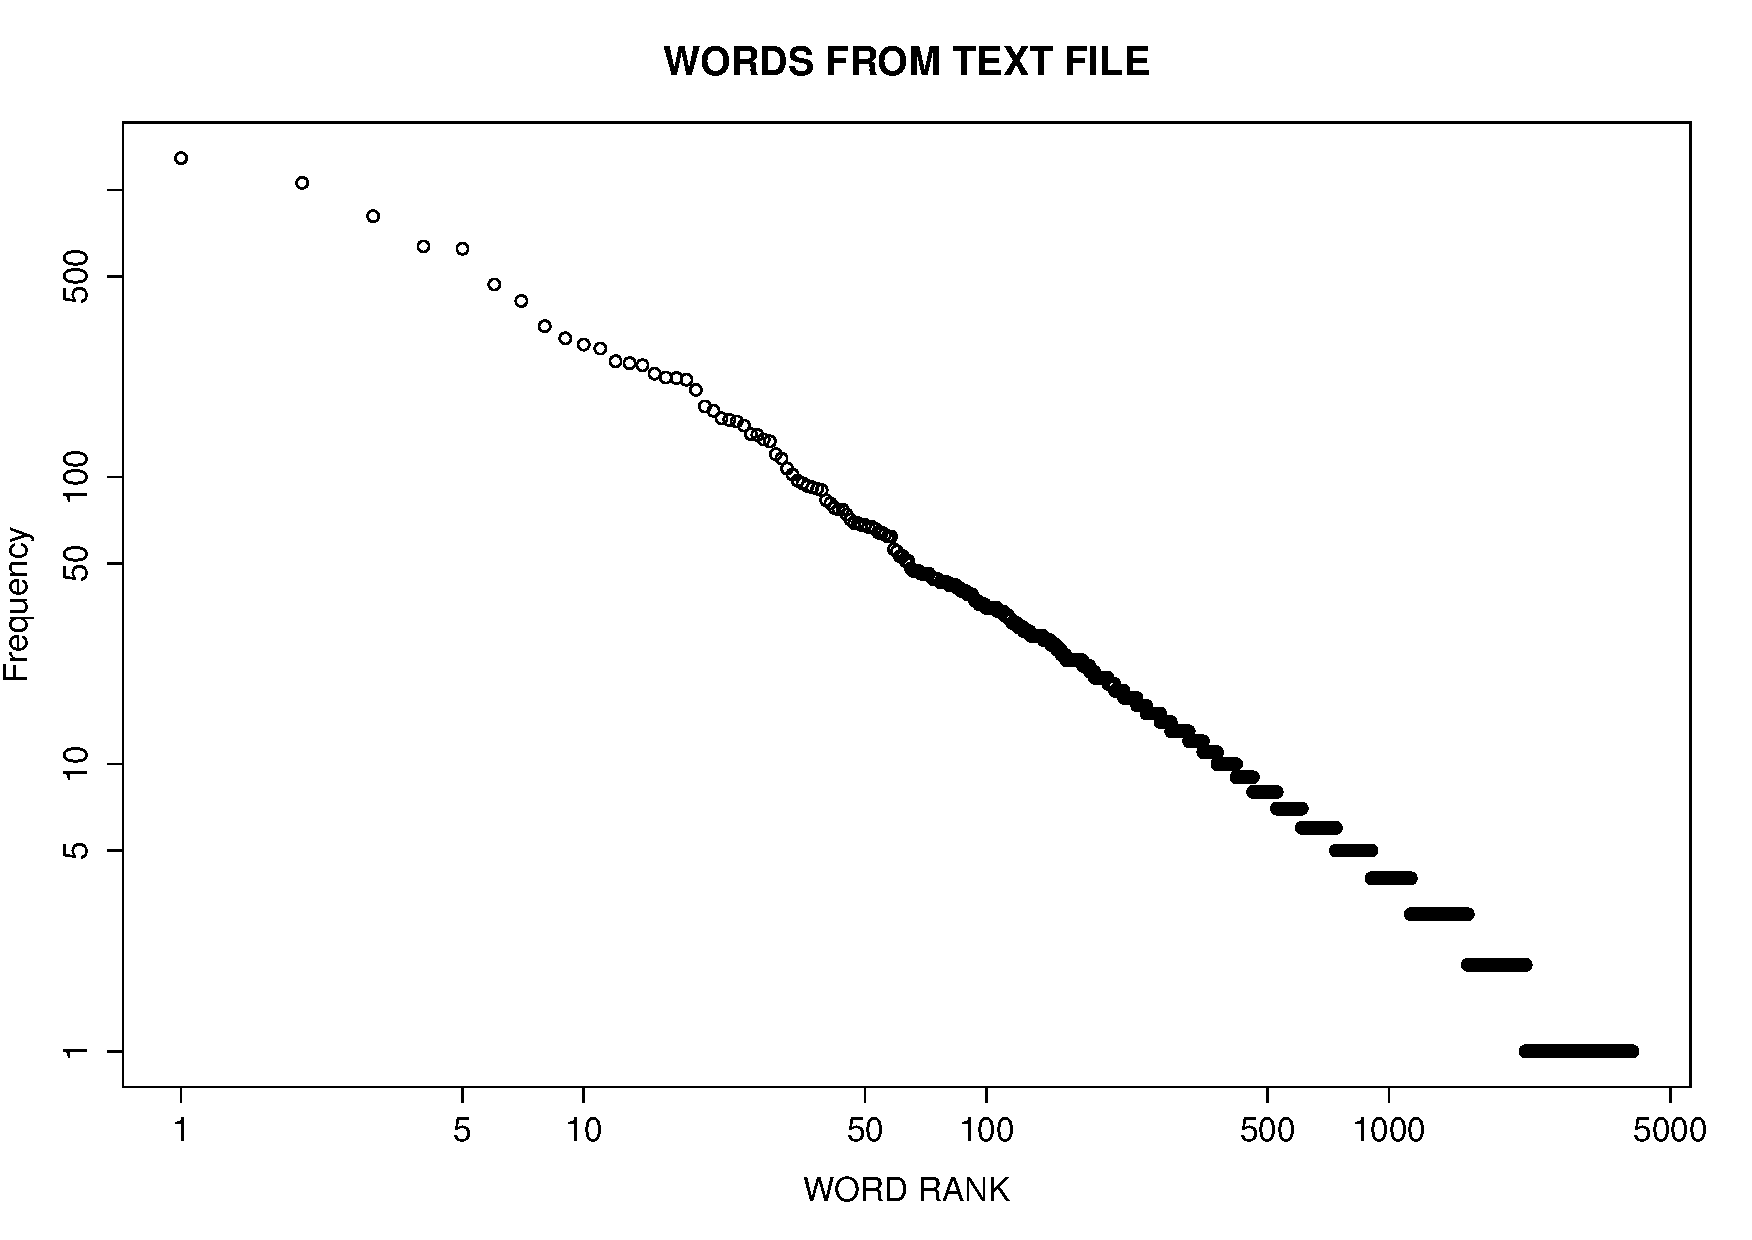
\includegraphics[width=0.8\columnwidth]{RplotTextZipf} % Example image
\end{center}



\begin{center}
{Figure 4: GRAPH TO PROVE Zipf’s LAW}
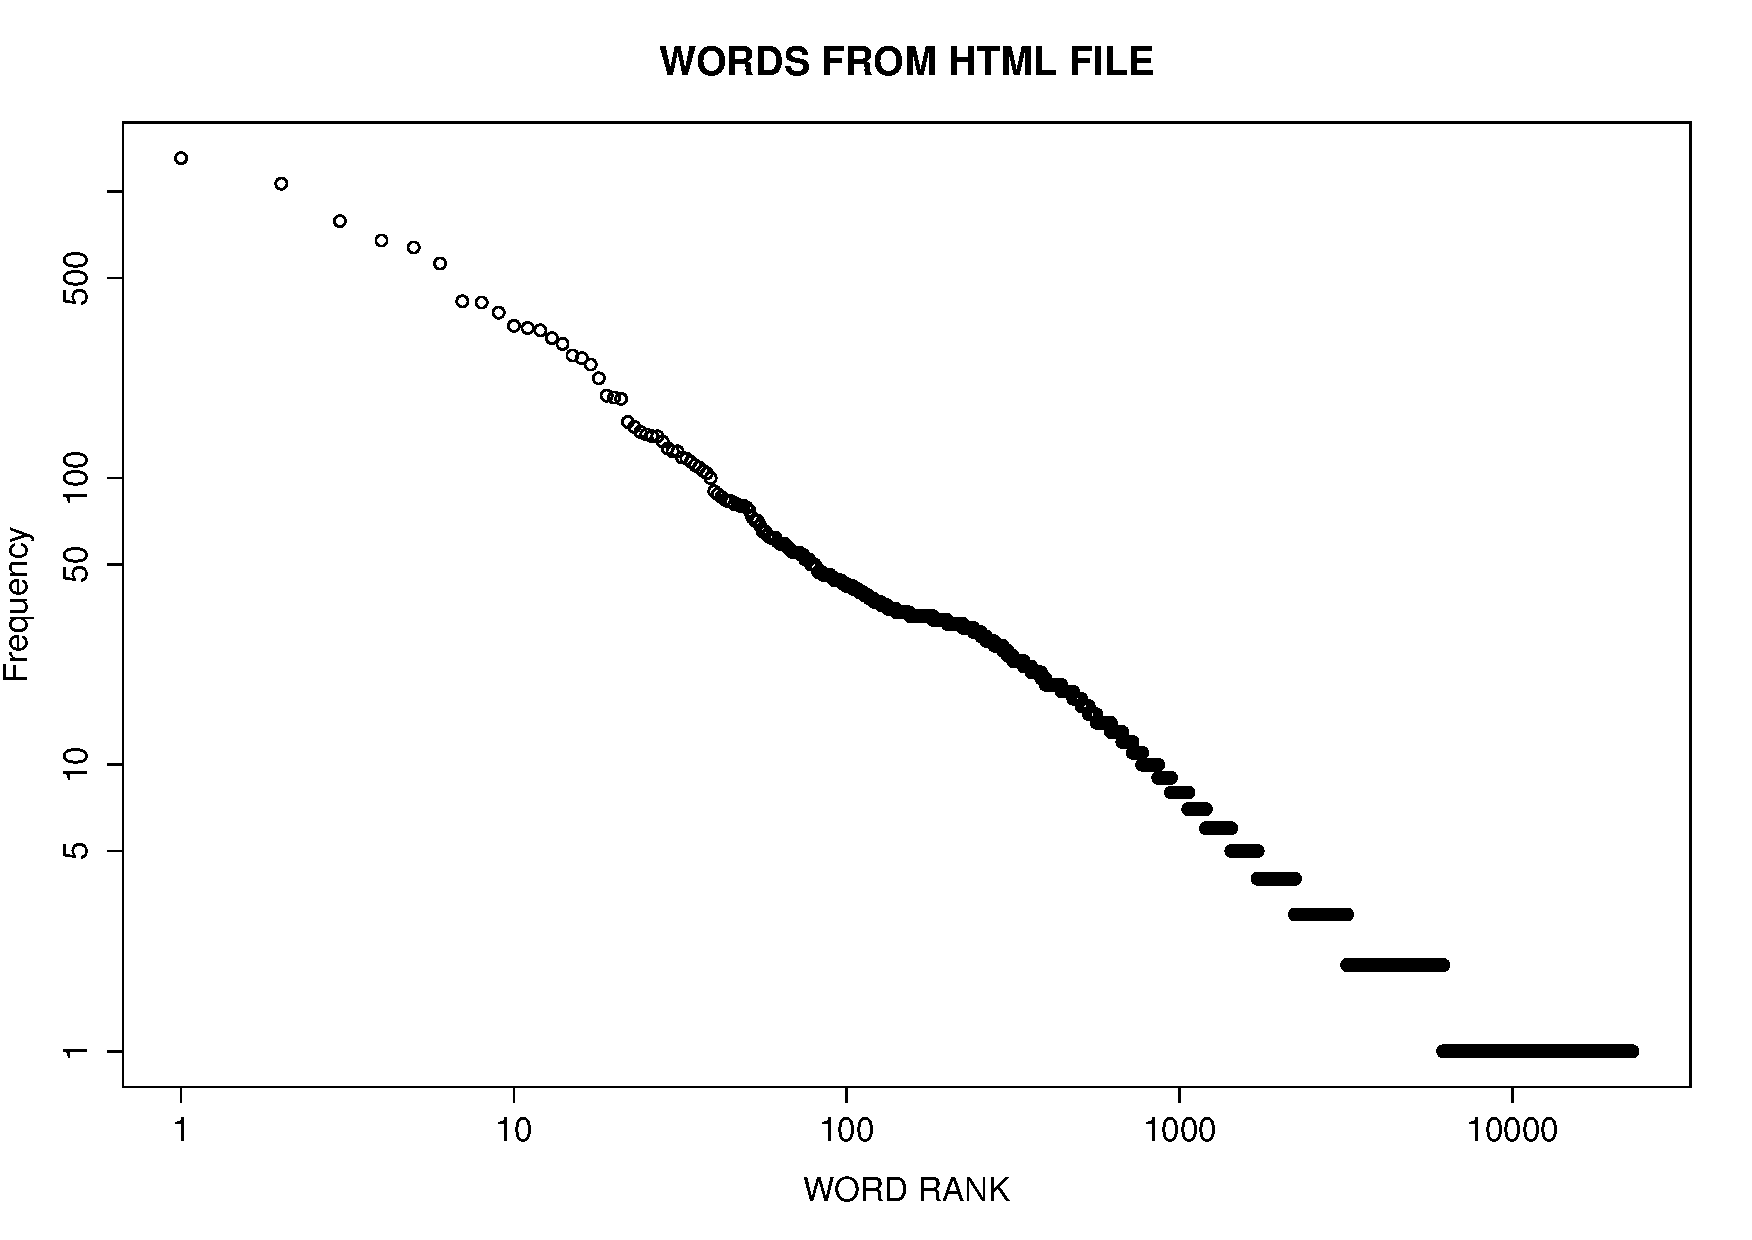
\includegraphics[width=0.8\columnwidth]{RplotHtmlZipf} % Example image
\end{center}

Using the stop word list I found that my first 50 words gotten form my text file had 47 stop words while the top 50 words gotten from HTML file had 42 stop words.
\newline
I also found that both graphs from the two collections follow the power law distribution . The classic almost perfect L-shape on the log-log scale is a dominant feature of power law graphs. I could not fully come to the absolute conclusion if the graph follows Zipf distribution, but this is what I discovered: Zipf's law is generally understood to simply be a power-law distribution with integer values. 
But, power-law distributions have the special property that the complementary cumulative distribution function (ccdf) is also a power law form. This presents some ambiguity in interpreting what exactly people mean when they state that the estimated such-and-such graph distribution or parameter follows Zipf's Law.

\end{homeworkProblem}

\newpage
%------------------------------------------------------------------
%  Bibilography
%------------------------------------------------------------------
\bibliographystyle{plain}
\bibliography{assignment_3}
\cite{*}
%----------------------------------------------------------------------------------------

\end{document}